
\section{Getting started}\label{sect:start}\ind{PISM!getting started}

In this section we give an extended example applying PISM to the Greenland ice sheet.  We use recent data sets provided by the Sea-level Response to Ice Sheet Evolution (\href{http://websrv.cs.umt.edu/isis/index.php/SeaRISE_Assessment}{SeaRISE}), a community-organized process to produce an upper bound of ice sheet contributions to sea level in the next 100--200 years.  For more about SeaRISE, see
\medskip

\centerline{\protect{\textbf{\url{http://websrv.cs.umt.edu/isis/index.php/SeaRISE_Assessment}}}}
\medskip

The example in this section is a quick, hands-on first look at PISM.  It is not an in-depth tutorial, and many details of what is happening will only be explained later.  The sections on the older EISMINT-Greenland and EISMINT-Ross modeling cases, for instance, do a more complete job of explaining the ways users will need to preprocess not-so-clean input data and then make-and-evaluate modeling choices.

The model output figures in this section were produced using a supercomputer.  In order for the examples here to run on a typical workstation, however, a rather coarse $20\,\textrm{km}$ grid is used.  The purpose of PISM is to make much higher spatial resolution actually possible, but it requires non-trivially \emph{parallel} processing.


\subsection{Install PISM}

See the \emph{Installation Manual} to install PISM.  Once installed, an executable \verb|pismr|, and several others, will be in the \verb|bin| subdirectory of the PISM directory.  For instance, that directory might be at \verb|/home/username/pism-dev/|.  The instructions below assume you start from that PISM directory.  We also assume you are using a \verb|bash| shell or at least one that accepts \verb|bash| syntax.


\subsection{Obtain and preprocess the input data}

The NetCDF data file which we use for input is freely-available at, and is described by, this web page: 
\medskip

\centerline{\protect{\textbf{\url{http://websrv.cs.umt.edu/isis/index.php/Present_Day_Greenland}}}}
\medskip

\noindent The quickest way to get the file itself is to do

\verb|$ cd examples/searise-greenland|

\noindent The script \verb|preprocess.sh| downloads the present-day data set  \verb|Greenland_5km_v0.93.nc| and adjusts it to make it PISM-readable.  If a different version number is desired, edit \verb|preprocess.sh| to change the line ``\verb|DATAVERSION=0.93|''.  Now run

\verb|$ ./preprocess.sh|

\noindent This downloads the present-day data and creates three NetCDF files, one of which has small ``metadata'' changes merely for PISM-readability, and the other two being separated time-dependent paleo-climate records from ice core and seabed core records.  (The ``present-day'' data actually includes some paleo-data!)

Any of these NetCDF files can be viewed with \verb|ncview| or other NetCDF visualization tool (see below).  Application of \verb|pyNGL| tools to \verb|Greenland_5km_v0.93.nc| produced figures \ref{fig:sr-input1} and  \ref{fig:sr-input1}, for example.  The metadata itself can be listed at the command line, or put in a text file, by \verb|ncdump -h|.

\begin{figure}[ht]
\mbox{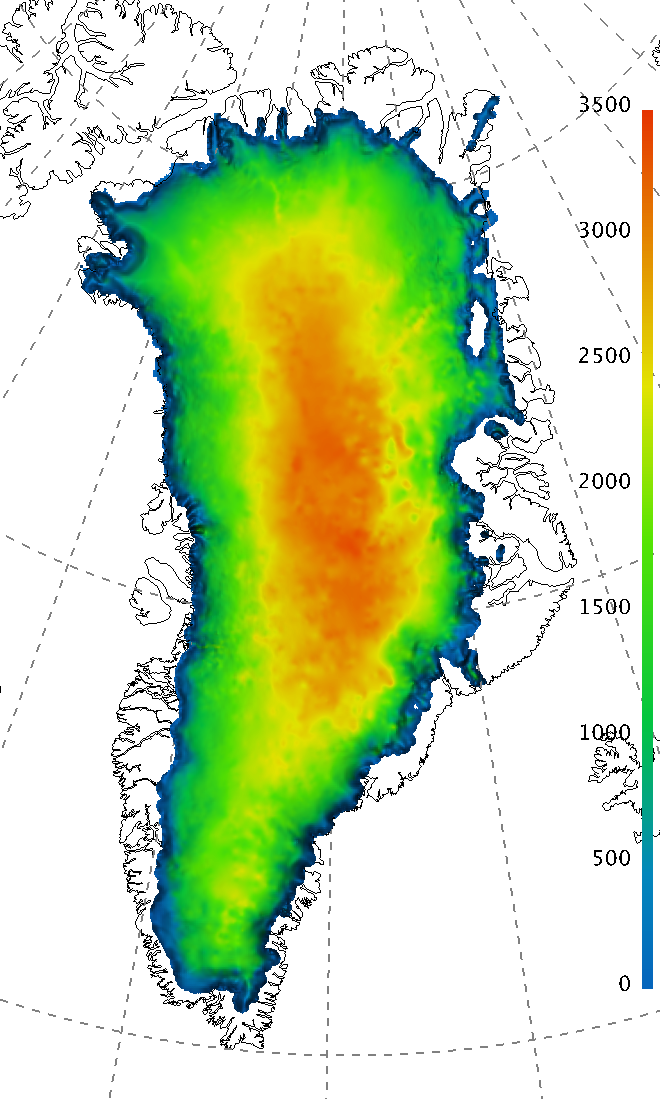
\includegraphics[width=3.0in,keepaspectratio=true]{sr-greenland-thk}
 \quad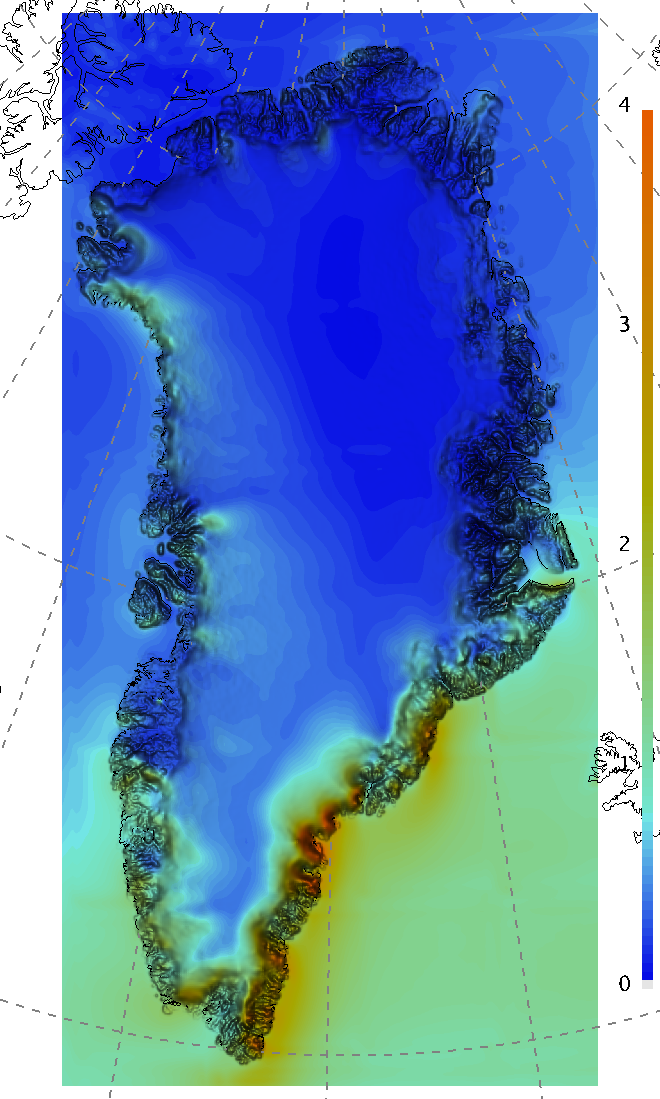
\includegraphics[width=3.0in,keepaspectratio=true]{sr-greenland-prcp}}
\caption{The input present-day ice thickness (left; m) and present-day precipitation (right; m $\text{a}^{-1}$ ice equivalent) for SeaRISE-Greenland.  Figures produced with FIXME: STATE TOOL}
\label{fig:sr-input1}
\end{figure}

\begin{figure}[ht]
\mbox{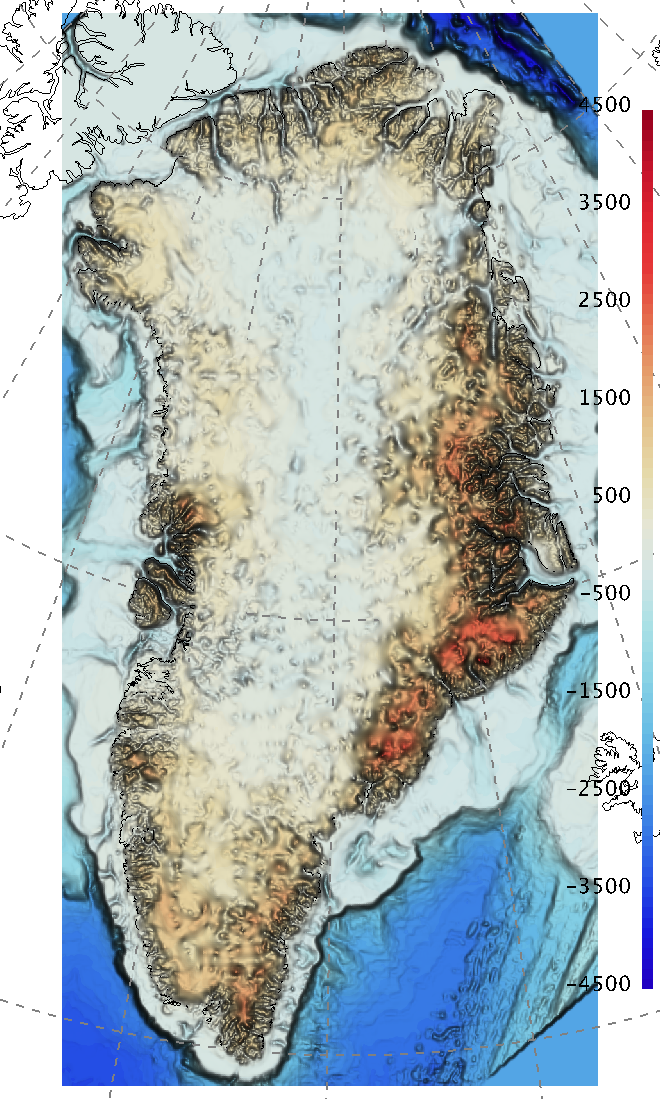
\includegraphics[width=3.0in,keepaspectratio=true]{sr-greenland-topg}
 \quad 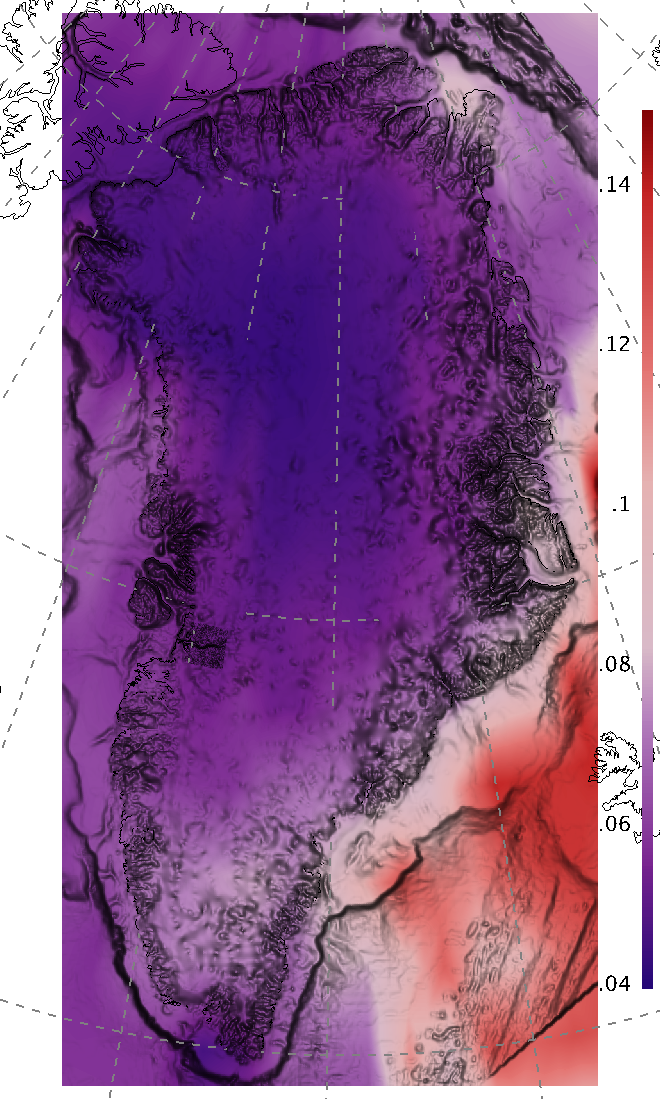
\includegraphics[width=3.0in,keepaspectratio=true]{sr-greenland-bheatflx}}
\caption{The input bedrock elevation (left; m) and geothermal flux (right; W $\text{m}^{-2}$) for SeaRISE-Greenland.  Figures produced with FIXME: STATE TOOL}
\label{fig:sr-input2}
\end{figure}


\subsection{Run PISM}

We are ready to run PISM, but, perhaps even more than many unix programs, PISM allows \emph{a lot} of command-line options.  In fact, because it is an ice flow simulation program designed to handle many different ice sheets, shelves, and glaciers, the list of user-configurable flags and parameters\footnote{At \protect{\textbf{\url{http://www.pism-docs.org/dev/doxy/html/config.html}}}}
is quite long.  We believe this is a \emph{feature} not a \emph{bug}!

For repeatably doing a major modeling job like SeaRISE-Greenland, it is, therefore, wise to build a \emph{script} to run PISM with the correct options.  Also, as explained in the rest of this \emph{User's Manual}, modeling ice sheets requires properly-integrating paleo-climatic and long-time-scale information into the model state, so our script is called ``\verb|spinup.sh|''.  The spin-up stage is the one which generally requires the most processor-hours.

To see what the SeaRISE-Greenland PISM run involves, do this:

\verb|$ export PISM_DO=echo|

\verb+$ ./spinup.sh+

\noindent Setting the environment variable \verb|PISM_DO| in this way tells \verb|spinup.sh| just to print out the commands it is about to run, not do them.

Note that ``\verb|mpiexec -n 2 pismr|'' appears in the echo-ed PISM runs from \verb|spinup.sh|.  This means that the PISM executable is run in parallel on two processes (e.g.~cores on a smaller machine).  For the rest of this example, we'll assume you have a typical year-2010 workstation with 8 cores.

The script \verb|spinup.sh| starts by ``bootstrapping.''  This means the creation, by heuristics and simplified models, of the kind of full initial conditions needed for the evolving, time-dependent model.  Specifically, the first run with 8 processes will look like
\begin{verbatim}
mpiexec -n 8 pismr -ocean_kill -skip 2 -boot_from pism_Greenland_5km_v0.93.nc \
  -Mx 76 -My 141 -Lz 4000 -Lbz 2000 -Mz 41 -Mbz 16 \
  -atmosphere searise_greenland -surface pdd -pdd_fausto \
  -y 100 -o g20km_pre100.nc
\end{verbatim}
This describes a 100 year run on a $76\times 141$ point grid in the horizontal, which is a 20 km grid.  There are also important choices about the vertical extent and resolution of the computational domain.



FIXME:  note total run time for complete 20km spinup r1043 on bueler-pogo, rank=8, was 104 processor-hours

\noindent This run should take about one minute of real time. Next we generate a more credible enthalpy field. One way to do this is to have the enthalpy field and velocity field co-evolve according to the thermomechanical flow model while holding the upper ice surface stationary.  This is a continuation of ``bootstrapping''.  The effect is to create an enthalpy field which is approximately stationary with respect to advection and conduction.\footnote{The resulting enthalpy field is not a fully physical enthalpy field, however, because it comes from a steadiness assumption about the geometry of the ice sheet.  Said another way, it is a enthalpy field in equilibrium with a velocity field for which the surface kinematical equation \cite{Fowler} is \emph{not} satisfied.}  We create this enthalpy field by running for 50000 years\footnote{A longer run might be desirabe, but here we only wish to have a reasonable starting field. More about how to determine the length of a no-mass run can be found in...} with non-evolving surface.  The option \verb|-no_mass| turns off the map-plane mass continuity scheme, and thus any evolution of the surface.
\begin{verbatim}
$ mpiexec -n 4 pismr -ocean_kill -skip 2 -i g20km_pre100.nc \
  -atmosphere searise_greenland -surface pdd -pdd_fausto -no_mass -y 50000 \ 
  -extra_file ex_g20km_steady.nc -extra_vars enthalpybase,temppabase \ 
  -extra_times 0:250:50000 -o g20km_steady.nc
\end{verbatim} This takes about 1 hour (4 processor hours). Before we proceed with the actual paleo-climate forcing, we add another short smoothing run:
\begin{verbatim}
$ mpiexec -n 4 /pismr -ocean_kill -skip 2 -i g20km_steady.nc \
  -atmosphere searise_greenland -surface pdd -pdd_fausto \
  -y 100 -o g20km_SIA.nc
\end{verbatim}



%%%%  OLD




PISM being parallel, it can be sped up by using more processes.  The standard output in \verb|out.eisIIA| can be tracked as the job is running in the background using \verb|less|\ind{less}, for instance.  Also, \verb|top|\ind{top} is a Linux tool to watch CPU and memory usage during the run.


To get the model state in the midst of a PISM run, send all running \verb|pisms| processes (the PISM executable used here) a signal which causes PISM to write out the model state: \verb|pkill -USR1 pisms|.\ind{PISM!catches signals -TERM and -USR1}\ind{USR1}\ind{pkill}  The PISM model state is then saved in a NetCDF file with name \verb|pism-|\emph{year}\verb|.nc|, using the year at that time step.  On the other hand, terminating the run with \verb|pkill -TERM pisms| will cause PISM to stop, but only after saving the model state using the specified output name.  See subsection \ref{subsect:signal} for a more complete description of how PISM catches signals.

While the complete run continues in the background, let's view the intermediate result stored in ...  An important fact to know is that a PISM output NetCDF file contains a ``history'' with the command that produced it.  For instance, 

\verb|$ ncdump -h simp_exper.nc|

\noindent This kind of ``history'' is convenient for understanding what you have done, once it all works!


Another way to view the output file is graphically.  One of the most convenient tools is \verb|ncview|; see Table \ref{tab:NetCDFview}.



As seen already, at each time step PISM shows a summary\ind{PISM!standard output summary of each time step} of the model state using a few numbers and some single character flags.  The format of the summary is partly explained by two lines near the beginning of the run:

\small\begin{quote}
\begin{verbatim}
P         YEAR:     ivol   iarea    meltf     thick0     temp0
U        years 10^6_km^3 10^6_km^2 (none)          m         K
\end{verbatim}
\end{quote}\normalsize

The ``\t{P}'' line is the prototype for the summary which appears at each time step.  The ``\t{U}'' line gives units for this summary.  From then on, the ``\t{S}'' lines give values for the quantities specified by the  ``\t{P}'' and ``\t{U}'' lines.

The EISMINT II runs above illustrate how the time-stepping in PISM adapts in order to maintain stability for its (mostly) explicit methods.  At the beginning of the EISMINT II run, for instance, the ice has small thickness so the time step is 60 years, simply because that is the default maximum time step.  Later in that run, after about 5000 years, the time step is made smaller because the flow is faster.

After the year, the next three entries in the summary report the volume of the ice in $10^6 \,\text{km}^3$, the area covered by the ice in $10^6\,\text{km}^2$, and the basal melt fraction, that is, the fraction of the ice area where the basal temperature is at the pressure-melting temperature.  This melted-base-fraction is a pure number without units.  The next two columns ``\texttt{thick0}'' and ``\texttt{temp0}'' are values at the center of the computational domain of the map plane, namely the ice thickness in meters and the absolute temperature of the ice at its base, in Kelvin.  These five numbers are the ones reported in the tables in \cite{EISMINT00}, which explains why they are the default quantities for reporting to standard output.  For more on the EISMINT II experiments see section \ref{sect:simp}.



\subsection{Handling NetCDF files}\label{subsect:nctoolsintro}  At a trivial level, PISM is just a program which takes a NetCDF file as input, does some computation, and produces a NetCDF file as output.  (An exception is that \verb|pisms| knows formulas to initialize EISMINT II experiments, for example.)  The user is in charge of creating NetCDF input files containing data on ice sheets worth modeling\footnote{See the section \ref{sec:bootstrapping-format} and table \ref{tab:modelhierarchy} for a hint about data necessary for modeling.}, and extracting some meaning from the NetCDF output files.

The most basic tools for converting NetCDF files to and from a standard text representation are called \verb|ncdump| and \verb|ncgen|.  A glance at Unix \verb|man| pages for these tools might be wise at this time.

As suggested earlier, we regularly use \verb|ncview| to look at NetCDF files.  The NetCDF tools most frequently used by the PISM developers are shown in Table \ref{tab:NetCDFview}.  This website gives additional NetCDF-related tools:

\centerline{ \href{http://www.unidata.ucar.edu/software/netcdf/docs/software.html}{\t{www.unidata.ucar.edu/software/netcdf/docs/software.html}} } 

\newcommand{\netcdftool}[1]{#1\ind{NetCDF!tools!#1}}
\begin{table}[ht]
\caption{Some tools for viewing and modifying NetCDF files.}\label{tab:NetCDFview} 
\small
\begin{tabular}{@{}llll}\hline
\textbf{Tool} & \textbf{Site} & \textbf{Function}\\ \hline
\netcdftool{\texttt{ncdump}} & \emph{included with any NetCDF distribution} & dump binary NetCDF as \texttt{.cdl} (text) file \\
\netcdftool{\texttt{ncgen}} & \emph{included with any NetCDF distribution} & convert \texttt{.cdl} file to binary NetCDF \\
\netcdftool{\texttt{ncview}} & \href{http://meteora.ucsd.edu/~pierce/ncview_home_page.html}{\texttt{meteora.ucsd.edu/$\sim$pierce}} & quick graphical view \\
\netcdftool{IDV} & \href{http://www.unidata.ucar.edu/software/idv/}{\t{www.unidata.ucar.edu/software/idv/}} & more complete visualization \\
\netcdftool{Paraview} & \href{http://www.paraview.org}{\t{www.paraview.org}} & powerful open-source parallel visualization \\
\netcdftool{NCL} &  \href{http://www.ncl.ucar.edu}{\t{www.ncl.ucar.edu}} & NCAR Command Language, open-source\\
\netcdftool{PyNGL} &  \href{http://www.pyngl.ucar.edu}{\t{www.pyngl.ucar.edu}} & Python version of NCL, open-source\\
\netcdftool{VisIt} & \href{http://visit.llnl.gov}{\t{visit.llnl.gov}} & advanced parallel visualization \\
\netcdftool{NCO}\ind{NCO (NetCDF Operators)} & \href{http://nco.sourceforge.net/}{\t{nco.sourceforge.net/}} & ``NetCDF Operators'': manipulations \\
\quad  & & \quad at command line
\end{tabular}
\normalsize
\end{table}


%%% Local Variables: 
%%% mode: latex
%%% TeX-master: "manual"
%%% End: 

